\documentclass[10pt,twocolumn,letterpaper]{article}

\usepackage{cvpr}
\usepackage{times}
\usepackage{epsfig}
\usepackage{graphicx}
\usepackage{amsmath}
\usepackage{amssymb}
\usepackage{xcolor}
\usepackage{subcaption}

% Include other packages here, before hyperref.

% If you comment hyperref and then uncomment it, you should delete
% egpaper.aux before re-running latex.  (Or just hit 'q' on the first latex
% run, let it finish, and you should be clear).
\usepackage[breaklinks=true,bookmarks=false]{hyperref}

\cvprfinalcopy % *** Uncomment this line for the final submission

\def\cvprPaperID{****} % *** Enter the CVPR Paper ID here
\def\httilde{\mbox{\tt\raisebox{-.5ex}{\symbol{126}}}}

% Pages are numbered in submission mode, and unnumbered in camera-ready
%\ifcvprfinal\pagestyle{empty}\fi
\setcounter{page}{1}
\begin{document}

%%%%%%%%% TITLE
\title{FocusFusion: Cross-Attention Fusion of LiDAR and Vision Features\\for 3D Semantic Segmentation}

\author{Edward Lee\\
Stanford University\\
{\tt\small edwardnl@stanford.edu}
\and
Saif Moolji\\
Stanford University\\
{\tt\small smoolji@stanford.edu}
\and
Umar Padela\\
Stanford University\\
{\tt\small umarp@stanford.edu}
}

\maketitle
%\thispagestyle{empty}

%%%%%%%%% ABSTRACT
\begin{abstract}
\par \noindent 3D semantic segmentation is a core perception task for autonomous driving, assigning each LiDAR point a semantic class label. While LiDAR provides geometric structure, it lacks the color, texture, and context clues in camera images. We propose FocusFusion, a multimodal architecture for nuScenes LiDAR semantic segmentation that fuses frozen LiDAR and camera representations using global cross-attention. We use LitePT to extract per-point geometric features from LiDAR and DINOv2 to extract patch-level visual embeddings from camera images. Rather than relying on explicit fusion techniques like projection, FocusFusion allows each LiDAR point to attend directly to image patch tokens, enabling the model to learn cross-modal correspondences from data. It also incorporates temporal context with the addition of a simple parameter-free memory bank that stores DINOv2 patch embeddings from the most recent keyframes. Only the cross-attention fusion module and segmentation head are trained, while the LiDAR and image backbones are frozen. We evaluate FocusFusion on nuScenes lidarseg and study the effects of Lovász-Softmax loss weighting, temporal depth, training data scale, and DINOv2 layer selection.
\end{abstract}

\section{Introduction}
Three dimensional semantic segmentation, which involves assigning a semantic class label to every point in a LiDAR scan, is a foundational perception problem for autonomous driving. Safe navigation demands that a vehicle not only know the geometry of its surroundings, but also the identity of each object, from road surfaces and lane dividers to pedestrians, cyclists, and traffic cones. Modern LiDAR sensors deliver precise depth and geometry, yet the point clouds they produce are inherently sparse in semantic information, since they carry no color, texture, or visual context such as signage or clothing that would help disambiguate objects with similar geometric structures - a thin vertical pole and a far-away pedestrian might look nearly identical in shape. Camera data, by contrast, capture rich appearance cues but lack the native ability to capture geometric information. Some existing approaches fuse LiDAR and image features via geometric projection and concatenation, mapping LiDAR points onto the image plane using known calibration matrices and appending the corresponding pixel-level features to each point ~\cite{xiao20243dopenvocabularypanopticsegmentation}. While effective as a baseline, this strategy is fundamentally limited by calibration accuracy, provides no mechanism for the model to discover useful correspondences, and offers no visual information for points that project outside the field of view or onto occluded regions.

In this work we propose FocusFusion, a fusion architecture that replaces projection-based feature retrieval with a learned global cross-attention mechanism. FocusFusion operates on two frozen foundation-model backbones: LitePT~\cite{litept2025}, which extracts per-point geometric features from the LiDAR scan, and DINOv2~\cite{oquab2024dinov2learningrobustvisual}, a vision transformer (ViT) that extracts spatially rich patch embeddings from each surround-view camera image. Each LiDAR point is free to attend to every image patch across all six cameras simultaneously, allowing the network to learn which visual regions are most informative for each point's classification, without the need for a calibration matrix. To incorporate temporal context, we maintain a simple parameter-free FIFO memory bank that stores DINOv2 patch embeddings from the most recent $T$ keyframes, enabling each point to draw on a short history of visual observations in case certain objects are occluded in the current frame. A lightweight MLP then maps the fused per-point features to one of 16 nuScenes semantic categories.

Our contributions are as follows: (1) a learned global cross-attention fusion of LiDAR and vision features requiring no calibration information at inference; (2) a parameter-free temporal patch memory bank aggregating DINOv2 embeddings over $T$ frames; and (3) ablation studies on the nuScenes lidarseg benchmark~\cite{caesar2020nuscenesmultimodaldatasetautonomous} over Lovász loss weight, temporal depth, training data scale, and DINOv2 feature layer selection, with attention map visualizations confirming meaningful cross-modal correspondences.

\section{Related Work}
Prior work on LiDAR-camera fusion for 3D semantic segmentation stems from combining LiDAR-only methods with camera-based 2D semantic segmentation and vision foundation models or temporal aggregation to preserve memory. Early methods such as PointNet use per-point multilayer perceptrons to segment raw point clouds \cite{qi2017pointnetdeeplearningpoint}, while PointNet++ adds hierarchical local grouping for improved performance \cite{qi2017pointnetdeephierarchicalfeature}. Voxel-based methods such as VoxelNet and SECOND discretize point clouds into voxel grids and apply 3D convolution, which improves long-range spatial context but can lose details on voxel boundaries \cite{zhou2017voxelnetendtoendlearningpoint, s18103337}. RandLA-Net addresses efficiency concerns for large outdoor scenes through random point sampling and local feature aggregation \cite{hu2020randlanetefficientsemanticsegmentation}, and Point Transformer V3 applies attention over point features for stronger geometric representations \cite{wu2024pointtransformerv3simpler}. We use LitePT as the LiDAR backbone \cite{litept2025}, a lightweight encoder that uses convolution blocks to capture local geometry before applying attention on a reduced set of point tokens, with PointROPE positional encoding to reduce computation and memory while achieving similar metrics to PTv3 — important given the cost of cross-attention over many LiDAR points and image tokens.

The DeepLab series uses dilated convolutions for dense 2D prediction \cite{chen2017rethinkingatrousconvolutionsemantic, chen2018encoderdecoderatrousseparableconvolution} and SegFormer uses an efficient transformer encoder for strong 2D segmentation performance \cite{xie2021segformersimpleefficientdesign}. Other camera-based approaches lift image features into 3D or bird's-eye-view (BEV) representations: Lift-Splat-Shoot predicts per-pixel depth distributions to project image features into BEV \cite{philion2020liftsplatshootencoding}, while BEVDet and BEVDepth extend this for camera-only 3D object detection \cite{huang2022bevdethighperformancemulticamera3d, li2022bevdepthacquisitionreliabledepth}, though all rely on accurate calibration and depth estimation.

CLIP learns image-language representations through contrastive pretraining, but its global image features are not well suited for dense spatial prediction \cite{radford2021learningtransferablevisualmodels}. DINOv2 is a self-supervised vision transformer that produces patch-level embeddings preserving local visual information while encoding high-level semantic structure \cite{oquab2024dinov2learningrobustvisual}, making it well suited for multimodal fusion; we use it as a frozen backbone to extract image patch features for cross-attention with LitePT.

PointPainting is a simple early-fusion approach that projects LiDAR points into the image plane and appends 2D semantic scores to each point feature \cite{vora2020pointpaintingsequentialfusion3d}, but depends directly on calibration accuracy and 2D segmentation quality. BEVFusion fuses LiDAR and camera features in a shared BEV representation to detect 3D objects \cite{liu2024bevfusionmultitaskmultisensorfusion}. GAFusion and DMFusion aggregate LiDAR-camera information across multiple frames and demonstrate the value of temporal multimodal fusion \cite{li2024gafusionadaptivefusinglidar, MA2025107572}. Waymo's 3D open-vocabulary panoptic segmentation shows the benefit of combining LiDAR encoders with 2D vision features through projection \cite{xiao20243dopenvocabularypanopticsegmentation}. Our approach instead uses learned cross-attention between LitePT point features and DINOv2 image patch features, allowing each LiDAR point to attend directly to visual tokens and learn correspondences from data rather than relying on projection or BEV pooling.

LiDAR-based temporal segmentation methods such as 4D Panoptic LiDAR Segmentation and SpSequenceNet accumulate point clouds across frames, improving geometric density and temporal consistency \cite{aygün20214dpanopticlidarsegmentation, 9156504}, while memory-based models such as XMem maintain features from previous frames to improve consistency and track objects \cite{cheng2022xmemlongtermvideoobject}. Inspired by these ideas, our parameter-free memory bank concatenates $T$ adjacent frames of DINOv2 patch embeddings to study whether temporal visual context improves dense LiDAR semantic segmentation without additional learned parameters.
% \subsection{LiDAR-Only 3D Segmentation}
% \begin{itemize}
%     \item \textbf{PointNet / PointNet++:} pioneered per-point MLP processing of raw point clouds; PointNet++ adds hierarchical local grouping; limitation: limited receptive field, no long-range context
%     \item \textbf{Voxel-based methods (VoxelNet, SECOND):} discretize points into a voxel grid and apply 3D convolutions; computationally scalable but lose fine-grained structure at voxel boundaries
%     \item \textbf{RandLA-Net:} random point sampling with local feature aggregation; efficient for large outdoor scans; still LiDAR-only, no semantic cues
%     \item \textbf{Point Transformer V3 (PTv3):} current state-of-the-art; uses space-filling curve serialization (Z-order / Hilbert) to impose a linear order on unstructured points, then applies window self-attention along that order; strong geometric representations pretrained on large indoor/outdoor datasets; \textbf{weakness:} no color, texture, or semantic cues from vision
%     \item \textbf{Gap:} all LiDAR-only methods struggle with texture-dependent classes (pedestrians, bicycles, traffic cones) where geometry alone is ambiguous
% \end{itemize}

% \subsection{Camera-Based Semantic Segmentation}
% \begin{itemize}
%     \item \textbf{DeepLab series:} dilated convolutions for dense 2D prediction; strong on RGB but produces 2D output with no depth
%     \item \textbf{SegFormer:} efficient transformer encoder for 2D semantic segmentation; lightweight and strong on standard benchmarks; inherits the 2D-only limitation
%     \item \textbf{Lift-Splat-Shoot (LSS):} lifts 2D image features to a 3D BEV representation via predicted per-pixel depth distributions; enables 3D reasoning from cameras; requires calibration and predicted depth is noisy
%     \item \textbf{BEVDet / BEVDepth:} camera-only BEV detection; effective for object detection but not designed for dense per-point semantic segmentation
%     \item \textbf{Gap:} camera-only approaches require accurate depth estimation or calibration to produce 3D outputs; do not natively annotate raw LiDAR points
% \end{itemize}

% \subsection{Multi-Modal LiDAR-Camera Fusion}
% \begin{itemize}
%     \item \textbf{PointPainting:} projects LiDAR points into the image plane, appends 2D semantic scores as additional point features; simple and effective early-fusion baseline; \textbf{weakness:} depends entirely on calibration accuracy and 2D segmentation quality
%     \item \textbf{BEVFusion (MIT / Nvidia):} fuses LiDAR and camera features in a shared BEV space; strong on 3D object detection; fusion happens at the BEV level rather than per-point, making dense per-point segmentation less natural
%     \item \textbf{GAFusion, DMFusion:} aggregate multi-frame LiDAR-camera features in BEV for 3D detection; demonstrate temporal fusion benefits; our work extends temporal vision fusion to dense semantic segmentation
%     \item \textbf{Waymo 3D open-vocabulary panoptic segmentation~\cite{Authors14}:} fuses LiDAR encoder with 2D vision features; foundational inspiration for our architecture; uses projection-based fusion rather than learned attention
%     \item \textbf{Our approach vs.\ prior work:} we replace projection / BEV pooling with \emph{global learned cross-attention} --- LiDAR points attend directly to image patch tokens with no geometric mask, learning correspondence from data; no calibration required at inference
% \end{itemize}

% \subsection{Vision Foundation Models for Perception}
% \begin{itemize}
%     \item \textbf{CLIP:} contrastive vision-language pretraining; powerful open-vocabulary global image features; patch-level spatial detail is limited compared to task-specific models
%     \item \textbf{DINOv2:} self-supervised ViT trained via self-distillation on curated internet images; produces spatially rich patch embeddings; shown to outperform supervised models on dense prediction tasks when used as a frozen backbone; \textbf{we use frozen DINOv2-small (ViT-S/14)}
%     \item \textbf{SAM (Segment Anything):} strong region-level segmentation; produces class-agnostic masks rather than semantic labels; not directly applicable to LiDAR point labeling
%     \item \textbf{Layer selection:} prior analysis shows DINOv2 layer 12 captures fine object detail while layer 9 captures broader region structure; we ablate both settings
% \end{itemize}

% \subsection{Temporal and Multi-Frame Methods}
% \begin{itemize}
%     \item \textbf{4D-PLS / SpSequenceNet:} extend LiDAR segmentation to temporal sequences by accumulating point clouds across frames; benefit from denser geometry but still LiDAR-only
%     \item \textbf{Video object segmentation memory networks (XMem, etc.):} maintain a memory of past frame features for consistent tracking; our memory bank is conceptually similar but operates on vision patch embeddings as keys/values for LiDAR-query attention
%     \item \textbf{Recurrent approaches:} ConvLSTM and similar architectures propagate hidden state across frames; add learnable temporal parameters; we deliberately keep our memory bank parameter-free (FIFO stack) to isolate the effect of temporal vision context
%     \item \textbf{Our memory bank:} stores the last $T$ sets of DINOv2 patch embeddings in a FIFO queue; $T=1$ is single-frame, $T=6$ covers 3 s at nuScenes 2 Hz keyframe rate; no additional learned parameters inside the bank
% \end{itemize}

\section{Method}

\subsection{Problem Formulation}

We formulate the problem as multimodal LiDAR semantic segmentation on nuScenes driving scenes. Given a LiDAR point cloud from the current timestep and a temporal window of camera observations of $T$ frames, we wish to predict the correct semantic category for each LiDAR point.

The input for a given timeframe $t$ consists of the LiDAR point cloud $P_t = \{p_{t,i} \in \mathbb{R}^4\}_{i=1}^N$ (x, y, z, and intensity) and a window of $T$ prior image frames $\{I_{t - T+1}, \dots, I_t\}$. The output is a per-point semantic prediction $\hat{y}_{t,i} \in \{1, \dots, C\}$ for each LiDAR point $p_{t, i}$, where $C = 16$ are the nuScenes lidarseg classes.

The objective is to learn a mapping between the input point cloud and image frames to the output per-point semantic labels of the LiDAR point cloud given by nuScenes as ground truth. In particular, we aim to combine geometric structure from the point cloud with visual semantic cues from the camera images to improve per-point segmentation accuracy.


\subsection{Architecture Overview}

Our architecture, as shown in Figure~\ref{fig:architecture}, first extracts features from the given point cloud and camera images. We use LitePT \cite{litept2025} as a frozen backbone to extract point cloud features and DINOv2 \cite{oquab2024dinov2learningrobustvisual} as a frozen backbone to extract image patch features. To create the image-based memory bank, we concatenate the last $T$ DINOv2 patch embeddings (including the current timestep) into a temporal window.

\begin{figure}
    \centering
    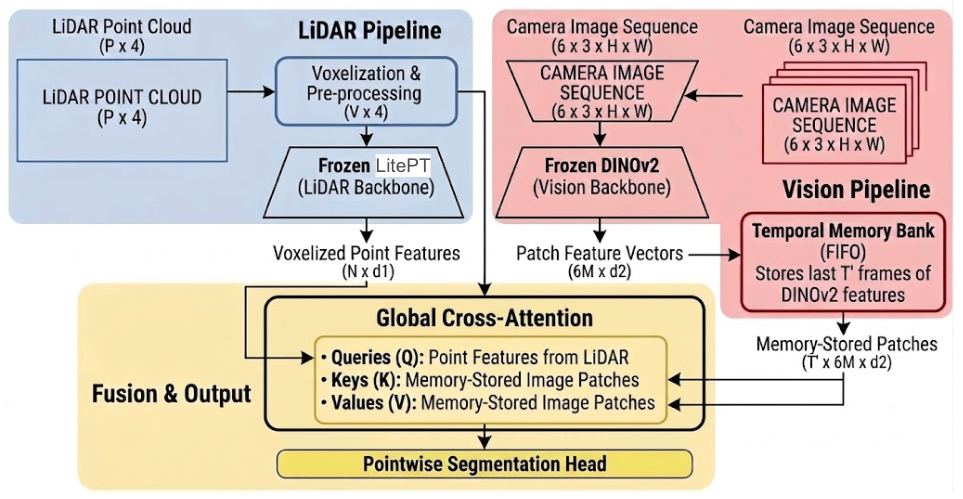
\includegraphics[width=0.9\linewidth]{architecture.png}
    \caption{FocusFusion Model Architecture}
    \label{fig:architecture}
\end{figure}

We then take these two branches and pass this into a global multi-head cross-attention layer, where LiDAR points query all vision patch tokens in the memory bank simultaneously. Finally, we pass the fused features through a lightweight MLP to get class logits for each point in the point cloud. Only the cross-attention fusion and MLP layers are trained, while the LitePT and DINOv2 backbones remain frozen.

% \begin{itemize}
%     \item \textbf{Two-branch design:} LiDAR branch extracts per-point features (PTv3 $\to$ $\mathbf{Q}$); Vision branch extracts patch embeddings per camera per frame (DINOv2 $\to$ memory bank $\to$ $\mathbf{K}, \mathbf{V}$)
%     \item \textbf{Fusion:} global multi-head cross-attention combines the two branches; LiDAR points query all vision patch tokens simultaneously
%     \item \textbf{Head:} lightweight MLP applied per point to fused features $\to$ class logits
%     \item Include architecture diagram figure here
% \end{itemize}

\subsection{LiDAR Backbone: LitePT}
We use LitePT as both the baseline we compare our results against and the LiDAR backbone for extracting the per-point geometric features of the input point cloud. LitePT is a lightweight point-transformer-style encoder designed to infer point-level representations using lower computational and memory cost than large LiDAR backbones. This is important for our project because these LiDAR features will be fused with image patch features through cross-attention, making computational efficiency a key design consideration.

The input to LitePT is an $N \times 4$ tensor, where each point is represented by its 3D coordinates and intensity. The backbone outputs a $N \times D_l$ ($D_l = 72$) tensor of per-point feature vectors, encoding the geometric structure of the point cloud compactly for downstream semantic segmentation. For our training, this backbone is kept frozen and used for the LiDAR-side query vectors $Q \in \mathbb{R}^{N \times D_l}$ in our cross-attention fusion module.

% \begin{itemize}
%     \item PTv3 serializes the unstructured point cloud using a space-filling curve (Z-order or Hilbert) to define a linear token order, then applies window self-attention along that sequence; avoids expensive $k$-NN graph construction
%     \item \textbf{Input:} $N \times 4$ tensor (x, y, z, intensity); \textbf{output:} $N \times D_l$ per-point feature vectors, $D_l = 256$
%     \item Pretrained on large indoor/outdoor datasets (ScanNet, S3DIS, nuScenes); provides strong zero-shot geometric representations
%     \item Fully frozen during training; per-point features become the query $\mathbf{Q} \in \mathbb{R}^{N \times D_l}$ for cross-attention
% \end{itemize}

\subsection{Vision Backbone: DINOv2}
We use DINOv2 (ViT-S/14) \cite{oquab2024dinov2learningrobustvisual} as our vision encoder. DINOv2 is trained via self-distillation without labels on a large-scale image dataset, yielding spatially rich patch-level embeddings that generalize well without fine-tuning. 

Each input image is divided into non-overlapping $14\times14$-pixel patches, producing $P$ patch tokens of dimension $D_v=384$. The model is run independently on all six camera images per timestep, yielding $6P$ patch tokens per time step. These tokens are passed to the temporal memory bank (Section~\ref{sec:membank}) and subsequently serve as keys and values in cross-attention. 

We use the final transformer block (layer 12) by default, as it captures fine-grained object-level detail. In an ablation, we concatenate layer-9 and layer-12 features, doubling $D_v$ to $768$ and incorporating broader region-level structure alongside local detail. The backbone is kept fully frozen throughout training.

\subsection{Temporal Memory Bank}
\label{sec:membank}
At each timestep, the patch tokens from the $T$ most recent time steps are concatenated to form the full key/value context $\mathbf{F}_v \in \mathbb{R}^{(T \cdot 6 \cdot P) \times D_v}$ passed to cross-attention. Setting $T=1$ uses only the current time step, while $T=6$ extends the context to 3 seconds of vision history at the nuScenes 2 Hz data rate. The memory bank introduces no learnable parameters, so the effect of temporal depth is isolated and studies through ablation of $T$ in section \ref{sec:temporal_depth}


\subsection{Cross-Attention Fusion}
We use the standard scaled dot-product multi-head cross-attention to fuse LitePT and DINOv2 tokens.
\[
    Q = F_l W_Q, \quad K = F_v W_K, \quad V = F_v W_V
\]
Here, $F_l \in \mathbb{R}^{N \times D_l}$ are PTv3 point features and $F_v \in \mathbb{R}^{(T\cdot 6 \cdot P) \times D_v}$ are stacked patch embeddings. We use global attention; we do not include any calibration mask or geometric constraint and allow every point to attend to every patch token.
% \begin{itemize}
%     \item Standard scaled dot-product multi-head cross-attention:
%     \[
%         \mathbf{Q} = \mathbf{F}_l \mathbf{W}_Q, \quad \mathbf{K} = \mathbf{F}_v \mathbf{W}_K, \quad \mathbf{V} = \mathbf{F}_v \mathbf{W}_V
%     \]
%     \[
%         \text{Attn}(\mathbf{Q}, \mathbf{K}, \mathbf{V}) = \text{softmax}\!\left(\frac{\mathbf{Q}\mathbf{K}^\top}{\sqrt{d}}\right)\mathbf{V}
%     \]
%     where $\mathbf{F}_l \in \mathbb{R}^{N \times D_l}$ are PTv3 point features and $\mathbf{F}_v \in \mathbb{R}^{(T \cdot 6 \cdot P) \times D_v}$ are stacked patch embeddings
%     \item Output $\in \mathbb{R}^{N \times d}$; each LiDAR point receives a weighted sum of all vision patch tokens
%     \item \textbf{Global attention:} every point attends to every patch token simultaneously; no calibration mask or geometric constraint
%     \item Learned $\mathbf{W}_Q, \mathbf{W}_K, \mathbf{W}_V$ are the only vision-fusion parameters trained end-to-end
%     \item Attention cost scales as $O(N \times T \times P)$; managed via point subsampling and mixed precision
% \end{itemize}

\subsection{Segmentation Head and Loss Functions}
To process the attention output, we train a simple 2-layer MLP head applied per point to output $C$-dimensional logits. Our total loss weights cross-entropy loss and the Lov\'{a}sz-Softmax loss \cite{berman2018lovaszsoftmaxlosstractablesurrogate}. The Lov\'{a}sz-Softmax directly optimizes the mIoU metric to address the class imbalances common in our data. Our total loss is calculated by
\[
    \mathcal{L}_{\text{CE}} = -\frac{1}{N} \sum_{i=1}^N \log p_{\hat{y}_i}(x_i)
\]
\[
    \mathcal{L}_{\text{Lov\'{a}sz}} =   \frac{1}{|C|} \sum_{c=1}^{C} \sum_{j=1}^{P} m_c^{(j)} \, \Delta_j(\mathbf{g}_c)
\]
\[
    \mathcal{L} = \mathcal{L}_{\text{CE}} + \lambda \mathcal{L}_{\text{Lov\'{a}sz}}
\]
Here, $m_c^{(j)} = |\mathbf{1}[y_i = c] - \hat{p}_{i,c}|$ are per-point softmax errors for class $c$ sorted in descending order, and $\Delta_j(\mathbf{g}_c)$ is the $j$-th component of the Lov\'{a}sz extension gradient, or the marginal increase in Jaccard loss when adding the $j$-th point. $\lambda \in \{
0, 0.25, 0.5\}$ is ablated.% \begin{itemize}
%     \item \textbf{Head:} 2-layer MLP applied independently per point to the fused features; outputs $C$-dimensional logits
%     \item \textbf{Cross-entropy loss:} $\mathcal{L}_{\text{CE}} = -\frac{1}{N}\sum_{i=1}^{N} \log p_{\hat{y}_i}(\mathbf{x}_i)$; standard per-point classification objective
%     \item \textbf{Lov\'{a}sz-Softmax loss:} a differentiable surrogate for the per-class Jaccard (IoU) score; directly optimizes the mIoU metric; particularly effective under class imbalance common in outdoor driving scenes
%     \item \textbf{Total loss:} $\mathcal{L} = \mathcal{L}_{\text{CE}} + \lambda \cdot \mathcal{L}_{\text{Lov\'{a}sz}}$, where $\lambda \in \{0,\, 0.25,\, 0.5\}$ is ablated
%     \item $\lambda = 0$ reduces to pure cross-entropy; $\lambda > 0$ adds an explicit IoU-maximization signal that benefits rare classes
% \end{itemize}

\section{Dataset and Features}

\subsection{nuScenes Dataset}
We evaluate FocusFusion on nuScenes, a large-scale autonomous driving dataset comprising $1000$ driving scenes collected across Boston and Singapore. Each scene spans approximately 20 seconds and is annotated at a keyframe rate of $2$ Hz. Every keyframe provides a synchronized 32-beam LiDAR sweep together with six surround-view camera images that collectively cover the full $360 ^\circ$ field of view around the vehicle. The lidarseg extension of nuScenes supplies per-point semantic labels on each keyframe LiDAR scan, originally annotated across 32 fine-grained categories. Since these categories end up with class labels that appear too infrequently in the dataset to be learned effectively, especially at this data scale, we follow the standard evaluation protocol of remapping these annotations to 16 semantic classes and exclude the noise class. The resulting label set spans common structural categories such as road, sidewalk, and vegetation, alongside safety-critical but slightly less frequently appearing objects such as pedestrian, bicycle, motorcycle, and traffic cone. As is typical of outdoor driving data, the class distribution is thus heavily imbalanced. Road and vegetation points dominate each scan, while rare classes may contribute only a small fraction of the total point count. This is the motivation for our use of the Lovasz-Softmax loss to explicitly optimize for per-class IoU. 

\subsection{Data Splits and Scale}

To study the effect of training data quantity on fusion quality we train on two subsets of the first portion of the full nuScenes training split (called blob1), which totals $70$ scenes composed of a sample of about $2800$ keyframes. The small-scale condition uses $10$ scenes, composed of approximately $400$ keyframes, randomly sampled from blob1 with a fixed seed for reproducibility. The large-scale condition uses all of the $70$ available scenes from blob1. We tune hyperparameters using blob1's own validation split for both conditions, and then report final test metrics on the nuScenes mini validation split, since it contains no overlap with either the train or validation splits for blob1 and was never used for hyperparameter tuning. When the temporal memory bank is active at depth $T$, the dataloader must supply $T$ consecutive keyframes from the same scene. We construct the temporal windows accordingly, and discard scenes shorter than the required window length.

\subsection{Preprocessing}
We take several preprocessing steps before training. On the LiDAR side, each raw point cloud is first voxelized at a grid resolution of $0.05$ meters using a first-point-per-voxel scheme, producing a set of sparse voxel coordinates and features that are passed into LitePT. Each voxel feature consist of the voxel's $(x, y, z)$ coordinates concatenated with the normalized intensity of its representative point, where the intensity is scaled from its raw $8$-bit value to $[0, 1]$ by dividing by $255$. Separately, the full point cloud is randomly subsampled to a fixed size of $N=16, 384$ points per keyframe to serve as the per point query inputs to the cross-attention module. When a scan contains fewer than $N$ points, the deficit is filled by sampling with replacement from the existing points. These padded points are assigned an label of $-1$, which is treated as the ignore index by the segmentation loss, so that they do not contribute to the gradient during training. Per point $(x, y, z)$ coordinates from this subsampled set form the spatial inputs, with corresponding inverse voxel indices used to retrieve LitePT features at inference. 

From the camera side, we resize each of the six surround-view images to $448 \times 448$ pixels, which are converted before training to a tensor in the range $[0,1]$. We normalize by the ImageNet mean and standard deviation prior to feature extraction. We use a ViT patch stride of $14$, which means each image yields $1024$ patch tokens. All features that are consumed by the fusion module are derived from these frozen backbones. LitePT produces 72-dimensional per point embeddings, and DINOv2 produces 384-dimensional patch embeddings.  


% \begin{itemize}
%     \item nuScenes is a large-scale autonomous driving dataset collected in Boston and Singapore; 1000 scenes of 20 seconds each at 2 Hz keyframe rate
%     \item Each keyframe provides a 32-beam LiDAR scan and 6 surround-view cameras with full 360\textdegree{} coverage
%     \item \textbf{lidarseg extension:} provides per-point semantic labels on keyframe LiDAR scans; 32 raw annotation categories remapped to 16 classes following standard protocol (noise/ignore class excluded)
%     \item Class distribution is highly imbalanced: road, vehicle, and vegetation dominate; pedestrians, bicycles, motorcycles, and traffic cones are rare but safety-critical
%     \item Cite: Caesar et al. (nuScenes), nuScenes lidarseg annotation extension
% \end{itemize}



% \subsection{Data Splits and Scale}
% \begin{itemize}
%     \item \textbf{Training data scale ablation:} we train on two subsets of the nuScenes training split --- 10 scenes ($\approx$400 keyframes) and 70 scenes ($\approx$2800 keyframes) --- to measure the effect of data quantity on fusion quality
%     \item \textbf{Validation:} fixed official nuScenes validation split used for all experiments; never used for hyperparameter selection
%     \item Include table: number of scenes / keyframes / total labeled points per split
%     \item The $T=6$ temporal window requires consecutive keyframes from the same scene; the dataloader collates windows accordingly
% \end{itemize}

% \subsection{Preprocessing}
% \begin{itemize}
%     \item \textbf{LiDAR:} points subsampled to $N \approx$ [fill in] per keyframe for compute tractability; coordinates normalized; intensity included as a fourth input channel to PTv3
%     \item \textbf{Images:} resized to [fill in] resolution (e.g., $518 \times 518$) compatible with DINOv2 ViT-S/14 patch size; standard ImageNet mean/std normalization applied
%     \item \textbf{Labels:} 32-class nuScenes annotations remapped to 16 categories; class 0 (noise) masked out of loss computation
%     \item No geometric data augmentation applied during training (potential future work)
%     \item \textbf{Features used:} raw per-point PTv3 embeddings ($D_l = 256$) and DINOv2 patch embeddings ($D_v = 384$ or $768$); no handcrafted features (HOG, SIFT, etc.)
% \end{itemize}

\section{Experiments, Results, and Discussion}

\subsection{Implementation Details and Hyperparameters}
In our implementation, we use Pytorch as a framework and train on A100 GPUs using Modal. We optimize using AdamW with a constant learning rate of $3 \times 10^{-4}$ and weight decay of \_. We trained with a batch size of four over 80 epochs, checkpointing after each epoch and selecting the checkpoint with the best validation mIoU. For our cross-attention layer, our weight shapes were $W_Q \in \mathbb{R}^{}$, $W_K \in \mathbb{R}^{}$, and $W_V \in \mathbb{R}^{}$, with eight total heads. In our hyperparamter sweeps, we tested $\lambda \in \{0, 0.25, 0.5\}$ swept on the 10-scene split for temporal bank sizes of $T=1$ and $T=6$. We found $\lambda = 0.25$ to perform the best and froze this for all subsequent experiments. For training, we used a single fixed training/validation split from nuScenes lidarseg.

% \begin{itemize}
%     \item \textbf{Framework:} PyTorch; training on Modal cloud A100 GPUs
%     \item \textbf{Optimizer:} AdamW; cosine LR decay schedule with linear warmup; LR decay schedule also varied in the data-scale experiment to find best results
%     \item \textbf{Batch size / epochs:} [fill in]; checkpoint saved each epoch, best selected by val mIoU
%     \item \textbf{Cross-attention:} [fill in] heads, $d = $ [fill in] model dimension
%     \item \textbf{Hyperparameter tuning:} $\lambda \in \{0, 0.25, 0.5\}$ swept on the 10-scene split for both $T=1$ and $T=6$; best $\lambda = 0.25$ then frozen for all subsequent experiments
%     \item All backbone weights (PTv3, DINOv2) frozen throughout; only cross-attention projection weights and MLP head are trained
%     \item No cross-validation; single fixed train/val split from nuScenes
% \end{itemize}

\subsection{Evaluation Metrics}
We focus on three quantitative metrics:
\begin{itemize}
    \item Mean intersection over union (mIoU) is our primary metric; it calculates the overlap between the predicted segment and the actual ground truth for each class, divided by the total area (the union) of both. By taking the average of these scores across all 16 categories, we get a single value that represents the overall spatial accuracy of the model.
    \[
        \text{mIoU} = \frac{1}{C} \sum_{i=1}^C \frac{\text{TP}_i}{\text{TP}_i + \text{FP}_i + \text{FN}_i}
    \]
    Here, $\text{TP}_i$ is the number of points correctly predicted as class $i$, $\text{FP}_i$ is the number of points incorrectly predicted as class $i$, and $\text{FN}_i$ is the number of points that belong to class $i$ but were incorrectly predicted as another class.

    \item Mean per-class accuracy (mAcc) measures the "precision" of our predictions by calculating the total number of points correctly identified for a specific class divided by the total number of points that actually belong to that class. It tells us, on average, how much of each object the model managed to capture.
    \[
        \text{mAcc} = \frac{1}{C} \sum_{i=1}^C \frac{\text{TP}_i}{\text{TP}_i + \text{FN}_i} 
    \]

    \item Frequency-weighted IoU (fwIoU) weights the IoU of each class by how often it appears in the dataset, ensuring that the final score isn't unfairly dominated by the model's performance on common, easy-to-detect surfaces.
    \[
        \text{fwIoU} = \frac{1}{\sum_{i=1}^C f_i} \sum_{i=1}^C f_i \cdot \text{IoU}_i
    \]
    Here, $f_i$ is the point frequency of class $i$.
\end{itemize}
By combining these three metrics, we can ensure that our model is not only accurate in a general sense but also reliable in detecting the rare, high-stakes objects necessary for safe navigation.
% \begin{itemize}
%     \item \textbf{mIoU} (mean Intersection over Union): primary metric; $\text{mIoU} = \frac{1}{C}\sum_{c=1}^{C} \frac{\text{TP}_c}{\text{TP}_c + \text{FP}_c + \text{FN}_c}$; treats all classes equally regardless of frequency
%     \item \textbf{mAcc} (mean per-class accuracy): $\text{mAcc} = \frac{1}{C}\sum_{c=1}^{C} \frac{\text{TP}_c}{\text{TP}_c + \text{FN}_c}$; measures per-class recall balance
%     \item \textbf{fwIoU} (frequency-weighted IoU): $\text{fwIoU} = \frac{1}{\sum_c f_c}\sum_{c=1}^{C} f_c \cdot \text{IoU}_c$ where $f_c$ is the point frequency of class $c$; emphasizes common classes (road, vehicle)
%     \item All three metrics reported on the fixed nuScenes validation split; per-class IoU included in table for safety-critical rare classes (pedestrian, bicycle, motorcycle, traffic cone)
% \end{itemize}

\subsection{Baseline: LitePt vs.\ FocusFusion}
We evaluated the pretrained LitePT directly on the nuScenes validation set, and compared it against the best performing Focus-Fusion model (by mIoU), which used $T=1$, lovasz parameter $0.25$, and was trained on the full 70 scenes from blob1. This model also used the image features from layer 12 of DINOv2. The results can be seen in Table ~\ref{tab:baseline}, where it is clear that FocusFusion has significant gains over the baseline in mIoU and mAcc, while performing similarly, albeit marginally worse in fwIoU. This suggests that the additional image features FocusFusion uses help better capture the intricacies of the rarer classes, since, by incorporating image features, we now inflate the amount of information for each given LiDAR point, making it easier to learn to predict these classes.

\begin{table}
\begin{center}
\begin{tabular}{|l|c|c|c|}
\hline
Method & mIoU & mAcc & fwIoU \\
\hline\hline
LitePT & 0.606 & 0.808 & 0.911 \\
FocusFusion (best) & 0.810 & 0.876 & 0.903 \\
\hline
\end{tabular}
\end{center}
\caption{Comparison of PTv3-only baseline vs.\ best FocusFusion ($T=1$, $\lambda=0.25$, 70 scenes, layer 12) on the nuScenes validation split.}
\label{tab:baseline}
\end{table}

% \begin{figure*}[t]
% \begin{center}
% \fbox{\rule{0pt}{1.8in} \rule{.9\linewidth}{0pt}}
% \end{center}
% \caption{Per-class IoU for the best FocusFusion model ($T=1$, $\lambda=0.25$, 70 scenes, layer 12) on the nuScenes validation split. Classes are sorted by frequency. Dashed line shows the PTv3-only baseline IoU for each class.}
% \label{fig:per_class_iou}
% \end{figure*}

\subsection{Ablation: Lovasz Loss Weight}
We sweep $\lambda \in \{0, 0.25, 0.5\}$ with all other settings fixed, evaluating at $T=1$. Results are shown in Table \ref{tab:lovasz_ablation}. At $\lambda=0$, the model trains on cross-entropy alone, which optimizes per-point classification accuracy and is therefore dominated by the gradient signal from common classes such as road and vegetation. Adding Lovász-Softmax at $\lambda=0.25$ increases the weight of rarer classes, giving them a stronger training signal and improving mIoU from $0.639$ to $0.683$. Increasing to $\lambda=0.5$ yields no further mIoU gain ($0.681$) while noticeably degrading mAcc from $0.798$ to $0.783$, suggesting that an excessive Lovász weight begins to over-penalize misclassifications on dominant classes and destabilizes the balance between the two loss terms. We fix $\lambda=0.25$ for all subsequent experiments.

\begin{table}
\begin{center}
\begin{tabular}{|c|c|c|c|c|}
\hline
$T$ & $\lambda$ & mIoU & mAcc & fwIoU \\
\hline\hline
1 & 0    & 0.639 & \textbf{0.809} & 0.903 \\
1 & 0.25 & \textbf{0.683} & 0.798 & 0.909 \\
1 & 0.5  & 0.681 & 0.783 & \textbf{0.910} \\
\hline
\end{tabular}
\end{center}
\caption{Ablation of Lovász loss weight $\lambda$ for $T=1$ and $T=6$ on the nuScenes validation split. Best result per $T$ in \textbf{bold}.}
\label{tab:lovasz_ablation}
\end{table}

\subsection{Temporal Depth: T=1 vs.\ T=6}
\label{sec:temporal_depth}

We compare single-frame vision context ($T=1$) against the six-frame temporal window ($T=6$) at the optimal loss weight $\lambda = 0.25$, with all other hyper-parameters held fixed. As shown in Table ~\ref{tab:temporal}, $T=1$ and $T=6$ have very similar performance across the three metrics on the validation split, with $T=1$ very slightly outperforming in terms of mIoU.

We attribute the underperformance of the temporal module to several compounding factors. First, at this training scale, the cross attention module must learn to attend over a key/value sequence that is six times longer than in the case when $T=1$, without a proportional increase in training diversity to supervise that larger attention space. Second, camera motion and scene dynamics over a three-second window introduce genuine variation in patch embeddings across frames, since a pedestrian could have moved substantially, or a previously visible vehicle maybe have become occluded. Our initial hypothesis was that this greater breadth of information would allow the model to pick out relevant additional information even when it is blurred at particular moments, but it is also possible that this adds noise to the key/value context that the model needs to then learn to ignore, which makes it infeasible given the amount of data we train on to do so. Moreover, the increased sequence length will raise attention variance, so without sufficient training data to regularize this, the model may default to diffuse or less discriminative attention distributions. We thus expect the benefit of temporal context to become more pronounced when training on the full nuScenes dataset, where greater scene diversity would provide richer supervision for attending over longer key/value sequences. 

\begin{table}
\begin{center}
\begin{tabular}{|l|c|c|c|c|}
\hline
T & mIoU & mAcc & fwIoU & allAcc\\
\hline\hline
1 & \textbf{0.810} & 0.876 & 0.903 & 0.947\\
6 & 0.806 & 0.875 & \textbf{0.902} & 0.947 \\
\hline
\end{tabular}
\end{center}
\caption{Comparing metrics for $T=1$ and $T=6$, fixed $\lambda=0.25$. }
\label{tab:temporal}
\end{table}
% \begin{itemize}
%     \item $T=1$ vs.\ $T=6$ results read from Table~\ref{tab:lovasz_ablation} at $\lambda=0.25$; reported separately here for emphasis
%     \item \textbf{Finding:} $T=1$ outperforms $T=6$ overall
%     \item Discussion of why $T=6$ underperforms: (1) small training dataset makes it harder to learn attention over a much longer $K/V$ sequence; (2) no temporal positional encoding means the model cannot distinguish patch ordering across frames; (3) camera motion and scene dynamics over 3 s introduce noise in patch embeddings; (4) increased $K/V$ length raises attention variance without enough data to regularize it
%     \item Per-class analysis: check whether $T=6$ helps dynamic classes (moving vehicles, pedestrians) even if global mIoU is lower
% \end{itemize}

\subsection{Training Data Scale: 10 vs.\ 70 Scenes}
To isolate the effect of training data quantity, we train FocusFusion on a randomly sampled subset of 10 scenes from blob1 and on the full 70-scene blob1 split, evaluating both on the held-out nuScenes mini validation split at $\lambda = 0$, to ensure there is no instability caused by the Lovasz weight at so few training examples. Results are show in Figure  ~\ref{fig:10vs70} for both $T=1$. 

Scaling from $10$ to $70$ training scenes consistently improves mIoU across both temporal settings, with gains of $19.6\%$ in the test set mIoU for $T=1$. We also see gains in mAcc by $12.1\%$, while fwIoU and allAcc remain fairly comparable across the two training sizes. From Figure ~\ref{fig:10vs70class}, we can see that the reason for this is that the largest gains come from rarer classes, such as motorcycles and traffic cones, which go from being totally unidentifiable by the model at 10 scenes, to having reasonable accuracy at 70 scenes. This indicates that the model with few enough scenes just does not have enough data to learn those rarer classes yet. This falls in line with what we would expect, since the cross-attention fusion module introduces learned projection weights $W_Q$, $W_K$, $W_V$ that must discover correspondences between LiDAR point features and image patch embeddings from scratch, since both backbones are frozen and provide no pre-aligned signal across the two modalities. More diverse training scenes expose the module to a wider variety of objects and object appearances, viewpoints, and lighting conditions, providing richer supervision for these projections.

\begin{figure}[t]
\begin{center}
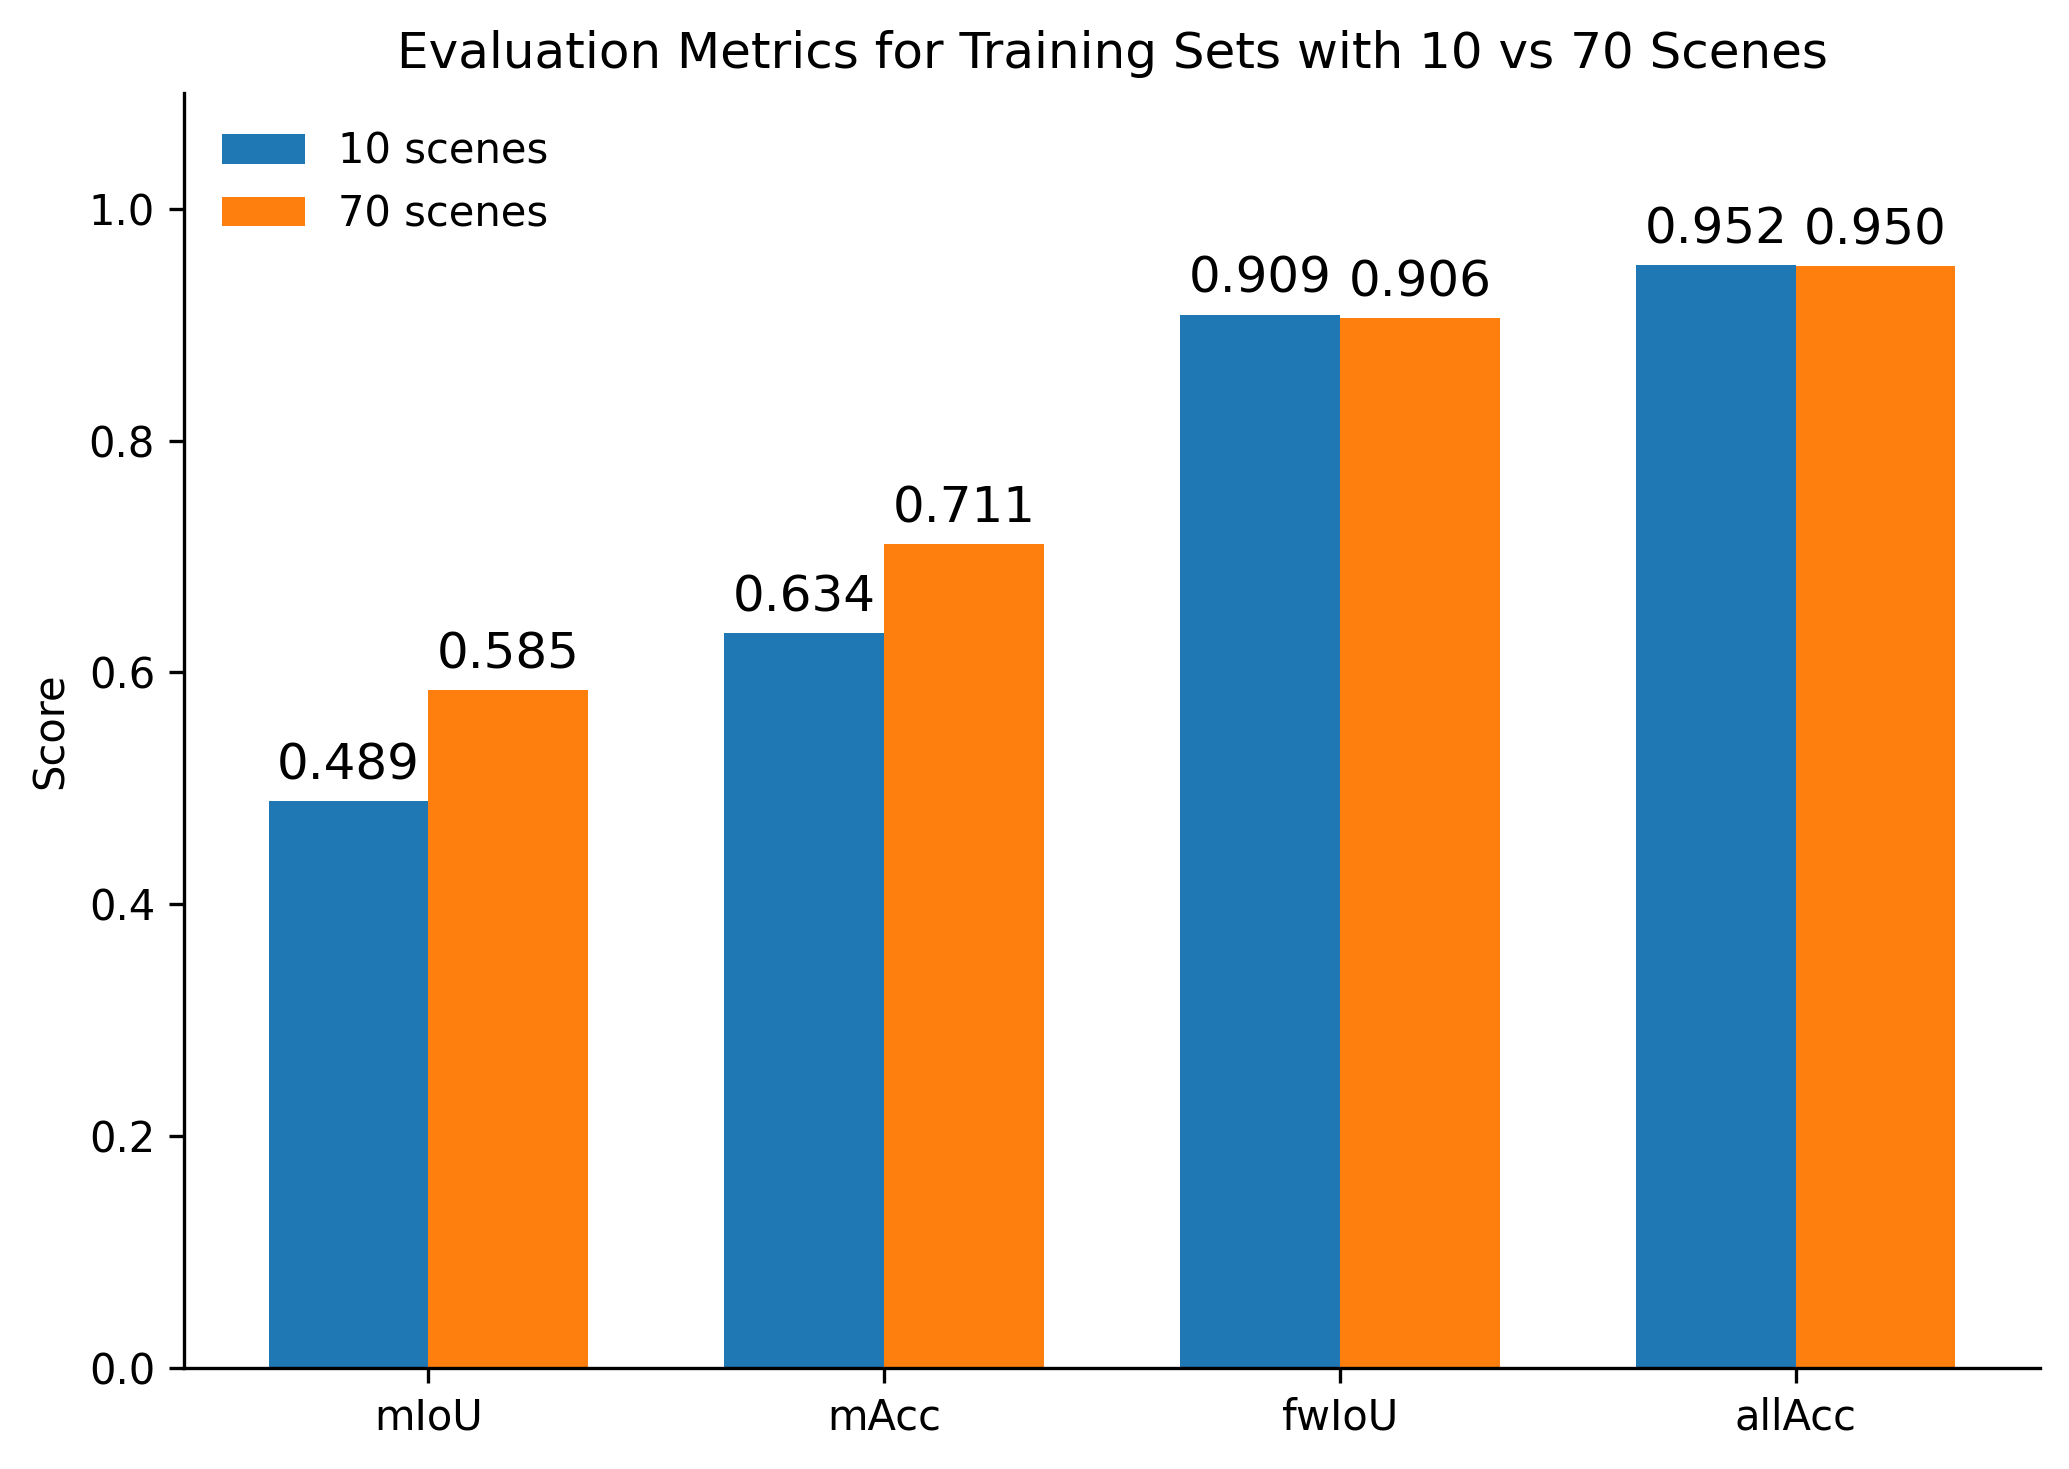
\includegraphics[width=0.9\linewidth]{train_size_figures/comparison_summary.png}
\end{center}
\caption{mIoU, mAcc, fwIoU, and allAcc (total accuracy) for $10$ scenes vs.\ $70$ scenes at $\lambda=0.0$ on the held out nuScenes mini validation split.}
\label{fig:10vs70}
\end{figure}

Inspecting training versus validation mIoU curves, the $10$-scene models show a notably larger train-val gap than the $70$-scene models, indicating overfitting at the smaller data scale. We can see in Table ~\ref{tab:miou_gap} that the gap in training and validation mIoU is far larger for the model trained on a smaller number of scenes. The cross-attention module and MLP head together constitute approximately $385$ thousand parameters, which, along with the backbone of the large pretrained vision and LiDAR experts, is enough capacity to memorize the small scene set. We apply dropout at $p=0.2$ and weight decay $= 10^{-3}$ throughout training as regularization, which partially mitigates the effect but does not eliminate it at 10 scenes. These results naturally suggest that the full goal should be to train on the entire nuScenes training split of $700$ scenes, and we expect the benefit of a larger $T$ to possibly emerge at that scale. 

\begin{table}[t]
\centering
\begin{tabular}{lccc}
\hline
\textbf{Setting} & \textbf{Train mIoU} & \textbf{Val mIoU} & \textbf{Gap} \\
\hline
10 scenes & $0.7195$ & $0.6364$ & $13.1\%$ \\
70 scenes & $0.8046$ & $0.7674$ & $4.8\%$ \\
\hline
\end{tabular}
\caption{Best training and validation mIoU (calculated on blob1 validation set) during training for 10-scene vs.\ 70-scene models. The generalization gap is computed as the percent difference between train mIoU and validation mIoU at the best validation epoch.}
\label{tab:miou_gap}
\end{table}

\subsection{DINOv2 Feature Layer Selection}

In a Vision Transformer, intermediate representations evolve from coarse to fine as depth increases: early layers encode broad region structure, grouping patches into large semantic zones such as sky, road surface, and background foliage, while later layers refine these into object-discriminative features with sharper boundaries. To guide our layer selection, we visualize DINOv2 patch embeddings from layers 9--12 using PCA, mapping the top three principal components to RGB in Figure~\ref{fig:dino_pca}. Layer 9 produces coarse color regions segmenting the scene at a high level, while layers 10 and 11 progressively sharpen these until, by layer 12, individual objects such as vehicles, pedestrians, and buildings are rendered as distinct, coherent regions.

Based on this analysis, we hypothesize that concatenating layer 9 and layer 12 features would provide complementary signals — layer 12 for precise object identity and layer 9 for broader scene context. Standard uses of DINOv2 concatenate all of layers 9--12, but we limit to these two since layers 10 and 11 blend between them, doubling $D_v$ from $384$ to $768$ while keeping the model lightweight.

Table~\ref{tab:dino_layer} shows the two configurations perform nearly identically: layers 9+12 achieves mIoU of $0.685$ versus $0.683$ for layer 12 alone. Given this negligible gain and the cost of doubling the key/value dimension, we adopt layer 12 only as our default. We attribute the indistinguishable performance to training scale: with 70 scenes, the cross-attention module likely lacks sufficient supervision to exploit the additional region-level signal from layer 9, which may become more valuable at the full nuScenes scale.



\begin{figure}[t]
\label{fig:dino_pca}
    \centering
    \begin{subfigure}[t]{0.31\linewidth}
        \centering
        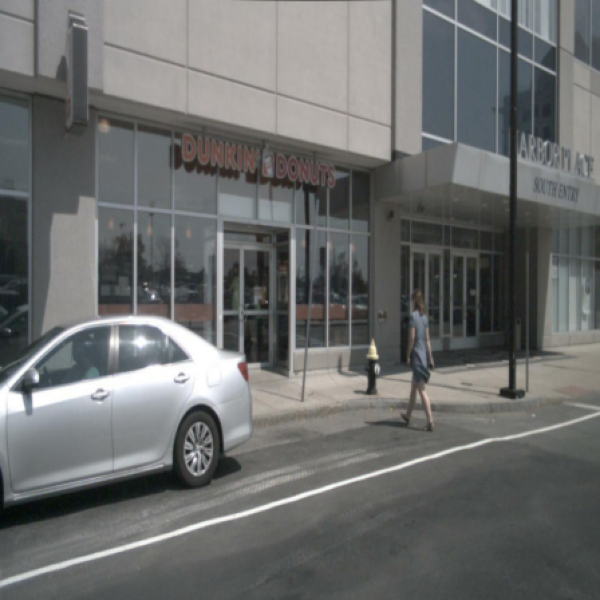
\includegraphics[width=\linewidth]{DINO_PCA/raw_img_DINO_PCA.png}
        \caption{Raw camera image}
        \label{fig:dino_raw}
    \end{subfigure}
    \quad
    \begin{subfigure}[t]{0.31\linewidth}
        \centering
        
\includegraphics[width=\linewidth]{DINO_PCA/layer9_DINO_PCA.png}
        \caption{Layer 9}
        \label{fig:dino_l9}
    \end{subfigure}
    \\[0.5em]
    \begin{subfigure}[t]{0.31\linewidth}
        \centering
        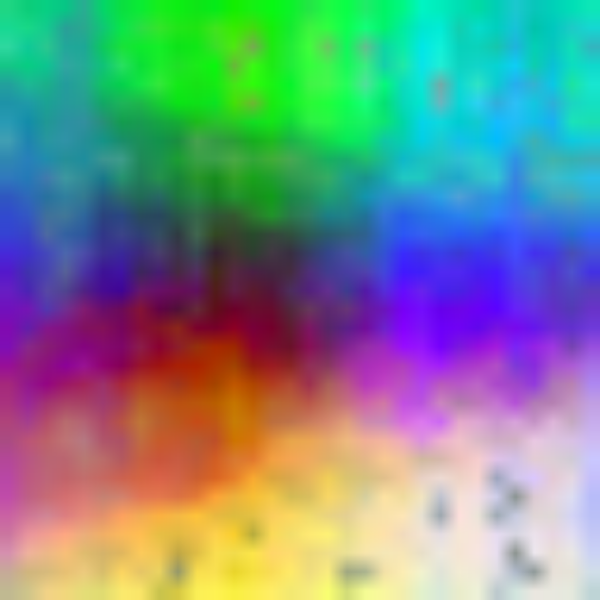
\includegraphics[width=\linewidth]{DINO_PCA/layer10_DINO_PCA.png}
        \caption{Layer 10}
        \label{fig:dino_l10}
    \end{subfigure}
    \hfill
    \begin{subfigure}[t]{0.31\linewidth}
        \centering
        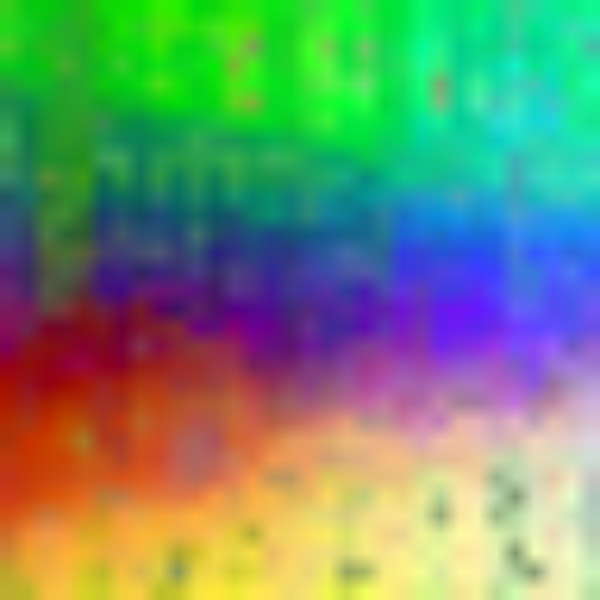
\includegraphics[width=\linewidth]{DINO_PCA/layer11_DINO_PCA.png}
        \caption{Layer 11}
        \label{fig:dino_l11}
    \end{subfigure}
    \hfill
    \begin{subfigure}[t]{0.31\linewidth}
        \centering
        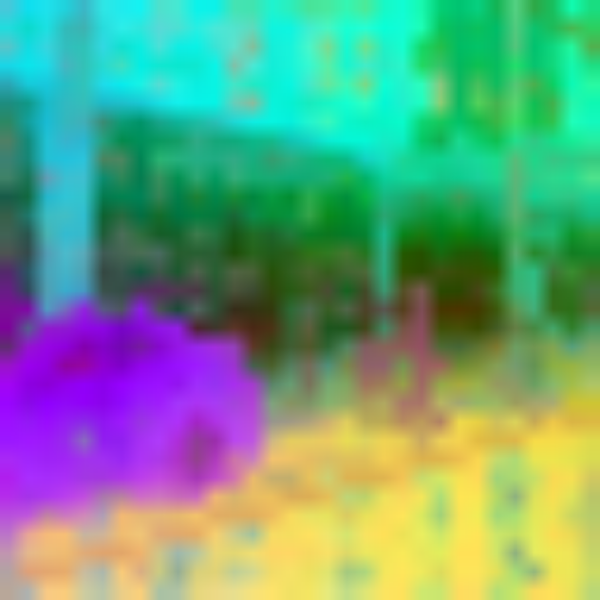
\includegraphics[width=\linewidth]{DINO_PCA/layer12_DINO_PCA.png}
        \caption{Layer 12}
        \label{fig:dino_l12}
    \end{subfigure}
    \caption{DINOv2 patch feature PCA visualizations across layers 9-12. Each image maps the top 3 principal components of patch embeddings to RGB, where distinct colors indicate semantically coherent regions.}
    \label{fig:dino_pca}
\end{figure}


\begin{table}
\label{tab:dino_tab}
\begin{center}
\begin{tabular}{|l|c|c|c|}
\hline
DINOv2 Features & mIoU & mAcc & fwIoU \\
\hline\hline
Layer 12 only ($D_v=384$)      & 0.683 & \textbf{0.798} & \textbf{0.909} \\
Layers 9+12 concat ($D_v=768$) & \textbf{0.685} & 0.782 & 0.907 \\
\hline
\end{tabular}
\end{center}
\caption{DINOv2 feature layer ablation at $T=1$, $\lambda=0.25$ on the nuScenes validation split.}
\label{tab:dino_layer}
\end{table}

\subsection{Qualitative Segmentation Results} 


\begin{figure}[t]
    \centering
    
    % --- SCENE 1: GROUND TRUTH ---
    \begin{subfigure}[b]{\linewidth}
        \centering
        % Limits height to 18% of the text page height, filling width up to aspect ratio
        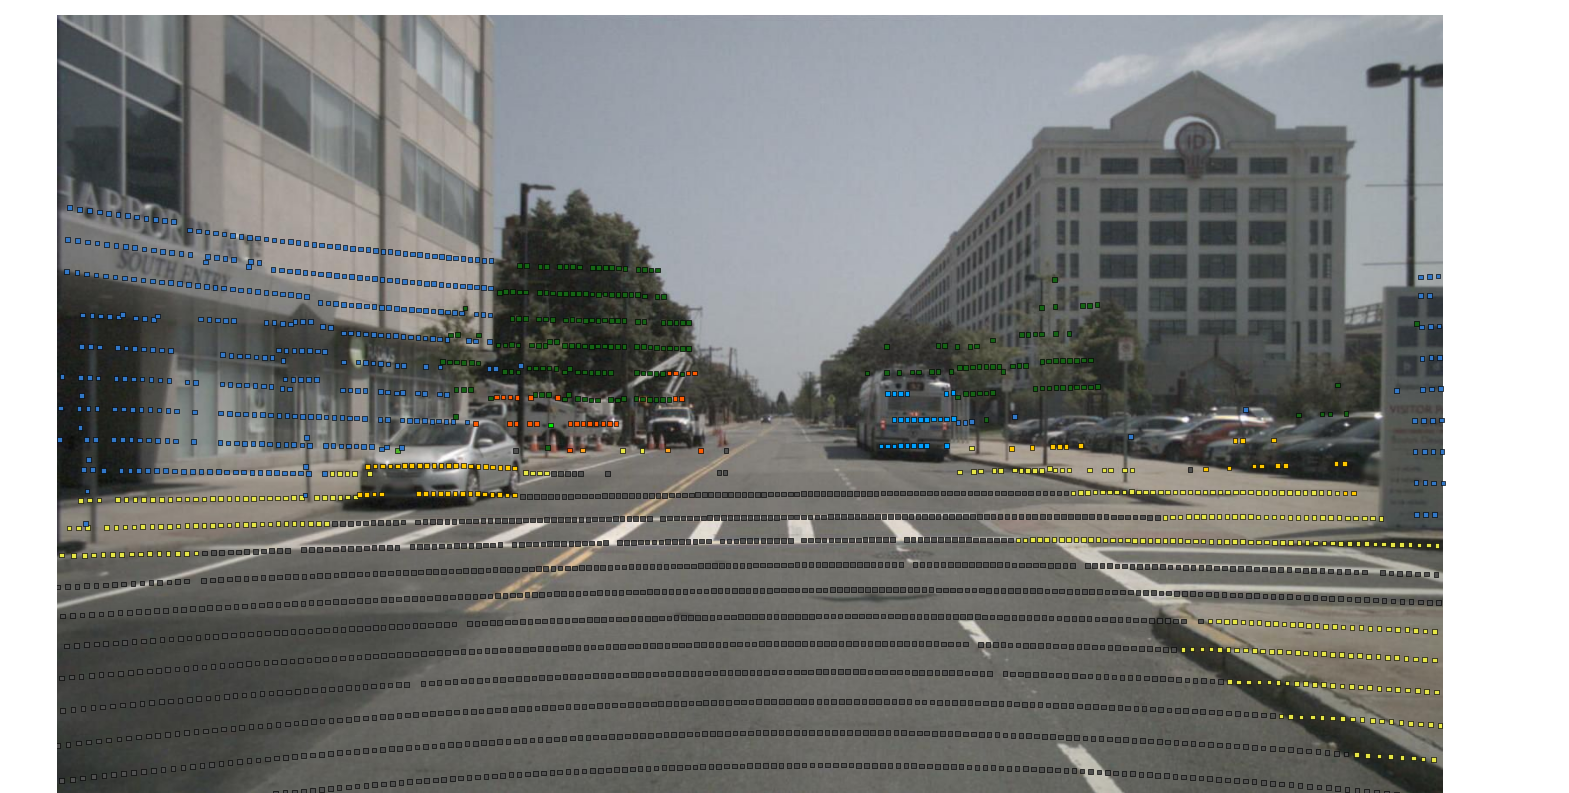
\includegraphics[width=\linewidth,height=0.18\textheight,keepaspectratio]{groundtruth_modal_comp/groundtruth1_cropped.png}
        \caption{Scene 1: Ground Truth}
        \label{fig:gt1}
    \end{subfigure}
    
    \vspace{0.2em}
    
    % --- SCENE 1: MODEL PREDICTION ---
    \begin{subfigure}[b]{\linewidth}
        \centering
        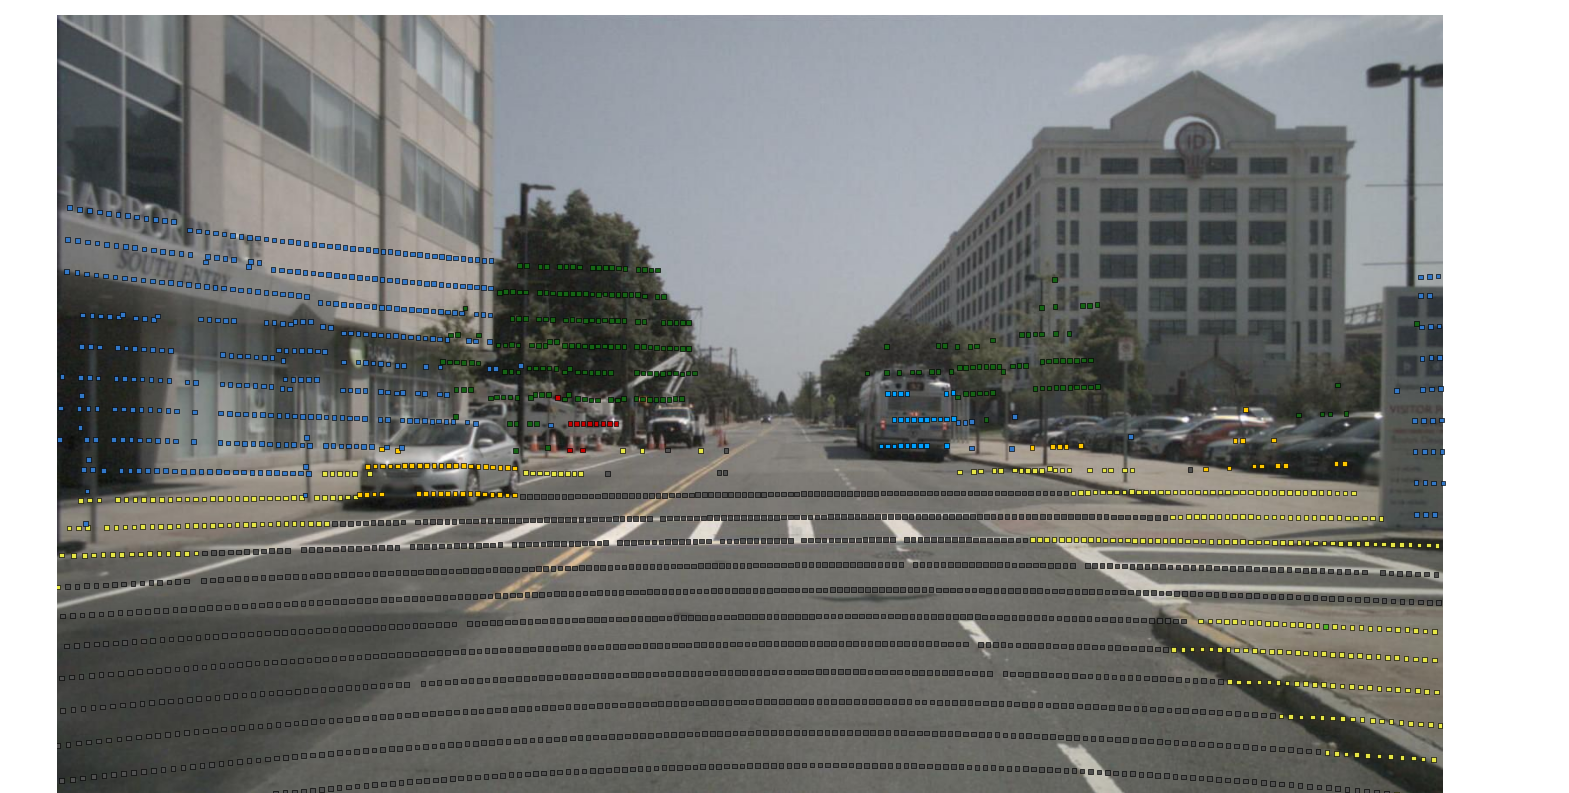
\includegraphics[width=\linewidth,height=0.18\textheight,keepaspectratio]{groundtruth_modal_comp/model1_cropped.png}
        \caption{Scene 1: Model Prediction}
        \label{fig:pred1}
    \end{subfigure}
    
    \vspace{0.1em}
    
\includegraphics[width=\linewidth]{groundtruth_modal_comp/legend1.png}
    
    \vspace{0.8em} % Moderate gap between distinct scenes


    \caption{Ground truth labels vs.\ model predictions for two validation scenes. LiDAR points are projected onto the front camera image and colored by semantic class.}
    \label{fig:qualitative}
\end{figure}

Figure~\ref{fig:qualitative} shows ground truth labels alongside FocusFusion predictions for two validation scenes, with LiDAR points projected onto the front camera image and colored by semantic class. The predictions are qualitatively coherent at a scene level - large structural categories such as road, vegetation, and vehicles are consistently segmented - but several recurring failure modes are apparent.

The most common error is the mislabeling of sidewalk points as terrain. These two classes are visually similar: both are flat, low-texture surfaces that appear in adjacent spatial regions of every scene, and the color and reflectance of concrete sidewalks and packed-earth terrain overlap considerably in the camera images. Because FocusFusion attends to image patch features for semantic context, this visual ambiguity is directly inherited: patches near the road boundary carry mixed appearance signals, and distinguish the two without sharper boundary cues or more training examples of each surface type in close proximity.

A second failure mode involves a tree in the foreground being mislabeled as a construction vehicle. In this scene, a construction vehicle is parked immediately behind the tree, and its patches dominate the image region that overlaps with the tree's LiDAR footprint. The model appears to attend to the truck patches rather than the foliage, assigning the construction vehicle label to points that geometrically belong to the tree. This is plausible for a cross-attention model with no geometric grounding: without calibration supervision, the model must learn from data alone which patches are relevant for each point. 

The reverse confusion also occurs: several points on the construction vehicle itself are labeled as vegetation, since surrounding tree canopy creates patches in the same image region. The two errors are thus symmetric, both stemming from the same underlying occlusion ambiguity between the tree and the truck.

Finally, traffic cone points are frequently mislabeled or ignored entirely. This is consistent with the per-class IoU results in Section~\ref{sec:temporal_depth}: traffic cones are small, rare, and visually distinctive only at close range, so the 70-scene training set provides insufficient examples for the fusion module to learn reliable cone-specific attention patterns. These failure cases collectively suggest that the primary bottleneck for FocusFusion's qualitative performance is training data diversity rather than a fundamental architectural limitation.


\section{Attention Map Visualizations}
To generate attention maps, we extract the cross-attention weight tensor $(H \times N \times S)$, average over the $H=8$ heads, and reshape into a $32 \times 32$ patch attention grid per camera. We select the camera with the highest total attention share for the query point, bilinearly upsample to full image resolution, and overlay as a heatmap where warmer colors indicate higher attention weight.

Figure~\ref{fig:attn_combined} shows two examples from the best-performing model ($T=1$, $\lambda=0.25$, 70 scenes, layer 12). For a terrain query point over short grass, attention is diffuse across the surrounding ground region, consistent with the homogeneous appearance of grass where many patches carry similar feature content. For a traffic cone query point, the model attends sharply to the cone's image patches, with its distinctive orange appearance producing a tight attention spike. However, overall traffic cone performance remains inconsistent: when a cone is small, distant, or occluded, the class's underrepresentation in training means the model often fails to activate this pattern, and misclassification is common. The success shown here reflects a favorable case rather than a general capability.

Together, these visualizations confirm that FocusFusion learns semantically meaningful cross-modal correspondences without geometric supervision or calibration, discovering relevant image regions purely from paired training data.
\begin{figure}[t]
    \centering
    \makebox[0.48\linewidth][c]{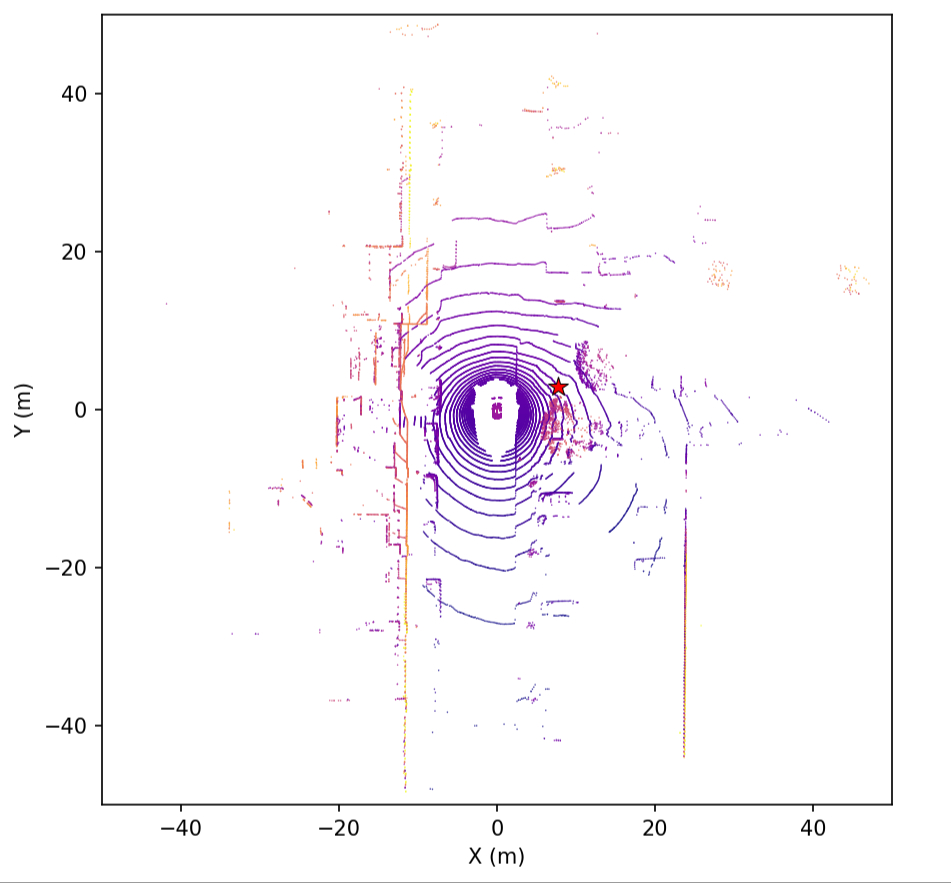
\includegraphics[height=3.5cm]{attention_map_figures/attention_map_terrain.png}}%
    \makebox[0.48\linewidth][c]{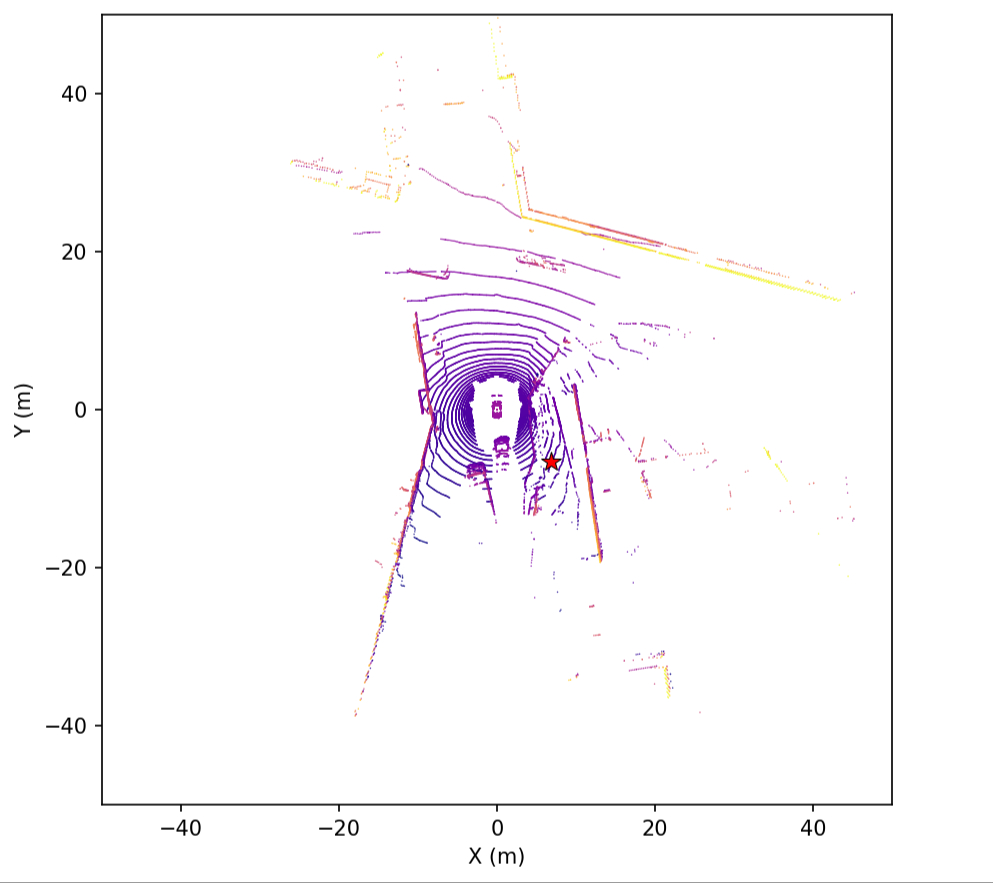
\includegraphics[height=3.5cm]{attention_map_figures/lidar_traffic_cone.png}}
    \\[2pt]
    {\small (a) LIDAR point clouds colored by height.}
    \vspace{0.5em}

    \makebox[0.48\linewidth][c]{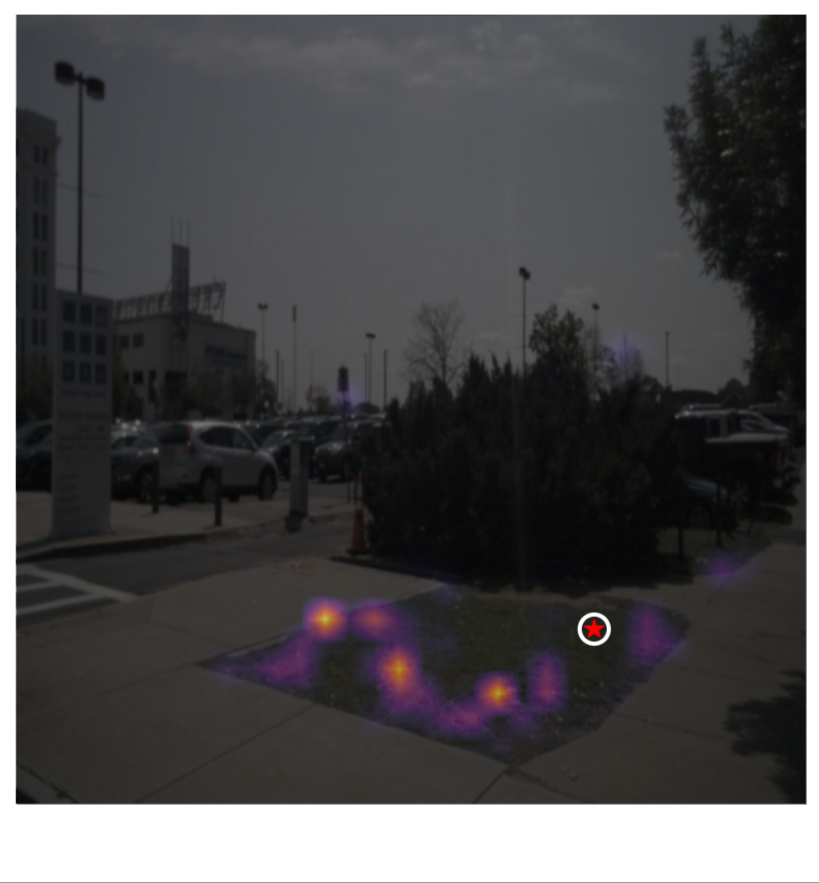
\includegraphics[height=3.5cm]{attention_map_figures/lidar_terrain.png}}%
    \makebox[0.48\linewidth][c]{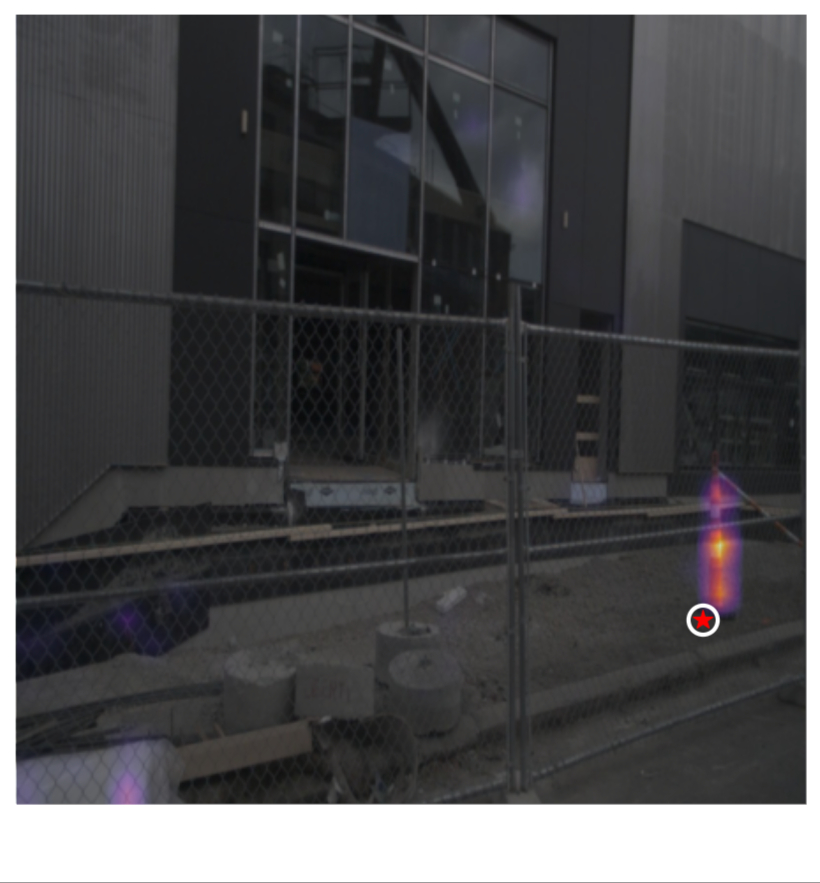
\includegraphics[height=3.5cm]{attention_map_figures/attention_map_traffic_cone.png}}
    \\[2pt]
    {\small (b) Cross-attention heatmaps; warmer colors indicate higher attention weight.}

    \caption{Attention visualizations for terrain (left) and traffic cone (right) query points. The model learns to attend to the relevant grass and traffic cone image patches.}
    \label{fig:attn_combined}
\end{figure}


\section{Conclusion and Future Work}
Our project, FocusFusion, demonstrates how learned global cross-attention can effectively fuse frozen LiDAR and vision features for 3D semantic segmentation without external information (e.g. camera-LiDAR calibration). In our experiments, we found that pure cross-entropy loss underperforms on rare classes and adding a Lovász-Softmax term to our loss improves performance (a weight of $\lambda = 0.25$ was best for us). We also found that the memory buffer did not perform as well compared to without it at our training scale, as $T = 1$ outperformed $T = 6$. This is likely due to the small training set proving insufficient to learn attention over the longer key-value sequences that $T = 6$ created. Additionally, we improved mIoU performance by scaling from 10 to 70 training scenes for both temporal settings. When processing the DINOv2 backbone, utilizing DINOv2 layer 12 alone is sufficient for training, as concatenating layer 9 yielded negligible gain. On the qualitative side, the attention maps confirm that there is semantically meaningful cross-modal correspondence.

In the future, we hope to train FocusFusion on the full nuScenes dataset of 700 scenes or the Waymo Open Dataset. We would expect that larger values of $T$ would improve in accuracy because there is enough data to learn attention for these longer sequences. Adding temporal positional embeddings or camera identity tokens to the memory bank might also assist with training on larger values of $T$. We could also finetune our LitePT or DINOv2 backbones on driving data (with a lower learning rate) for better performance. Another direction we could go is creating an attention mask that is inspired by projection to see if that helps training, or apply FlashAttention for memory-efficient long-sequence attention at large $T$. For robustness, we could test our model under degraded sensor inputs, such as night scenes, rain, or noisy LiDAR, to see if our fusion mechanism improves robustness in edge cases. Finally, we could extend our algorithm to train for panoptic segmentation, where we get both semantic and instance classification.

% \begin{itemize}
%     \item \textbf{Summary:} FocusFusion demonstrates that learned global cross-attention can effectively fuse frozen LiDAR (PTv3) and vision (DINOv2) features for 3D semantic segmentation without any camera calibration at inference
%     \item \textbf{Key findings:}
%     \begin{itemize}
%         \item $\lambda = 0.25$ Lovász loss weight is optimal; pure cross-entropy underperforms on rare classes
%         \item $T = 1$ (single-frame vision) outperforms $T = 6$ (3 s history) at this training scale
%         \item Scaling from 10 to 70 training scenes consistently improves mIoU for both temporal settings
%         \item DINOv2 layer 12 alone is sufficient; concatenating layer 9 yields negligible gain
%         \item Attention maps confirm semantically meaningful cross-modal correspondence is learned
%     \end{itemize}
%     \item \textbf{Why $T=6$ underperforms:} small training set insufficient to learn attention over long key/value sequences; absence of temporal positional encoding removes frame-ordering signal; future work should revisit with more data
%     \item \textbf{Future work:}
%     \begin{itemize}
%         \item Scale to full nuScenes (700 scenes) or Waymo Open Dataset; expect larger-$T$ benefit to emerge with more diverse training scenes
%         \item Add temporal positional embeddings and camera identity tokens to the memory bank
%         \item Fine-tune DINOv2 or PTv3 with a low learning rate for domain adaptation to driving data
%         \item Explore calibration-guided attention masking as an optional ablation
%         \item Apply FlashAttention for memory-efficient long-sequence attention at large $T$
%         \item Test robustness under degraded sensor inputs (night scenes, rain, LiDAR dropout)
%         \item Extend to panoptic segmentation (semantic + instance)
%     \end{itemize}
% \end{itemize}

\section*{Contributions and Acknowledgements }
Edward Lee worked on the LitePT backbone, ran the baseline metrics, and helped debug the fusion training script.

Saif Moolji worked on the fusion model and training scripts, conducted the temporal ablation studies, as well as the training set size studies. 

Umar Padela  worked on the DINOv2 backbone, ran the lovasz and DINO layer ablation studies, and generated the attention heatmaps, groundtruth and model visualizations, and DINO PCA analysis.

Everyone helped with writing the project proposal and final paper, as well as creating and presenting each of the milestones. Everyone will also assist with creating and presenting the poster for the poster session.

Generative AI was used to help generate a project\_plan.md file, and it was only used to organize our existing ideas, not to propose new ones. The project plan has a change log describing the changes and iteration we made on our ideas, while generative AI was used to summarize those ideas into the project plan. We also used it for advice on how to cut down portions of the paper since we were over the limit.

{\small
\bibliographystyle{ieee}
\bibliography{egbib}
}
\newpage 
\appendix
\section{Comparison per Label for 10 and 70 scene training sets}

\begin{figure*}[t]
\centering
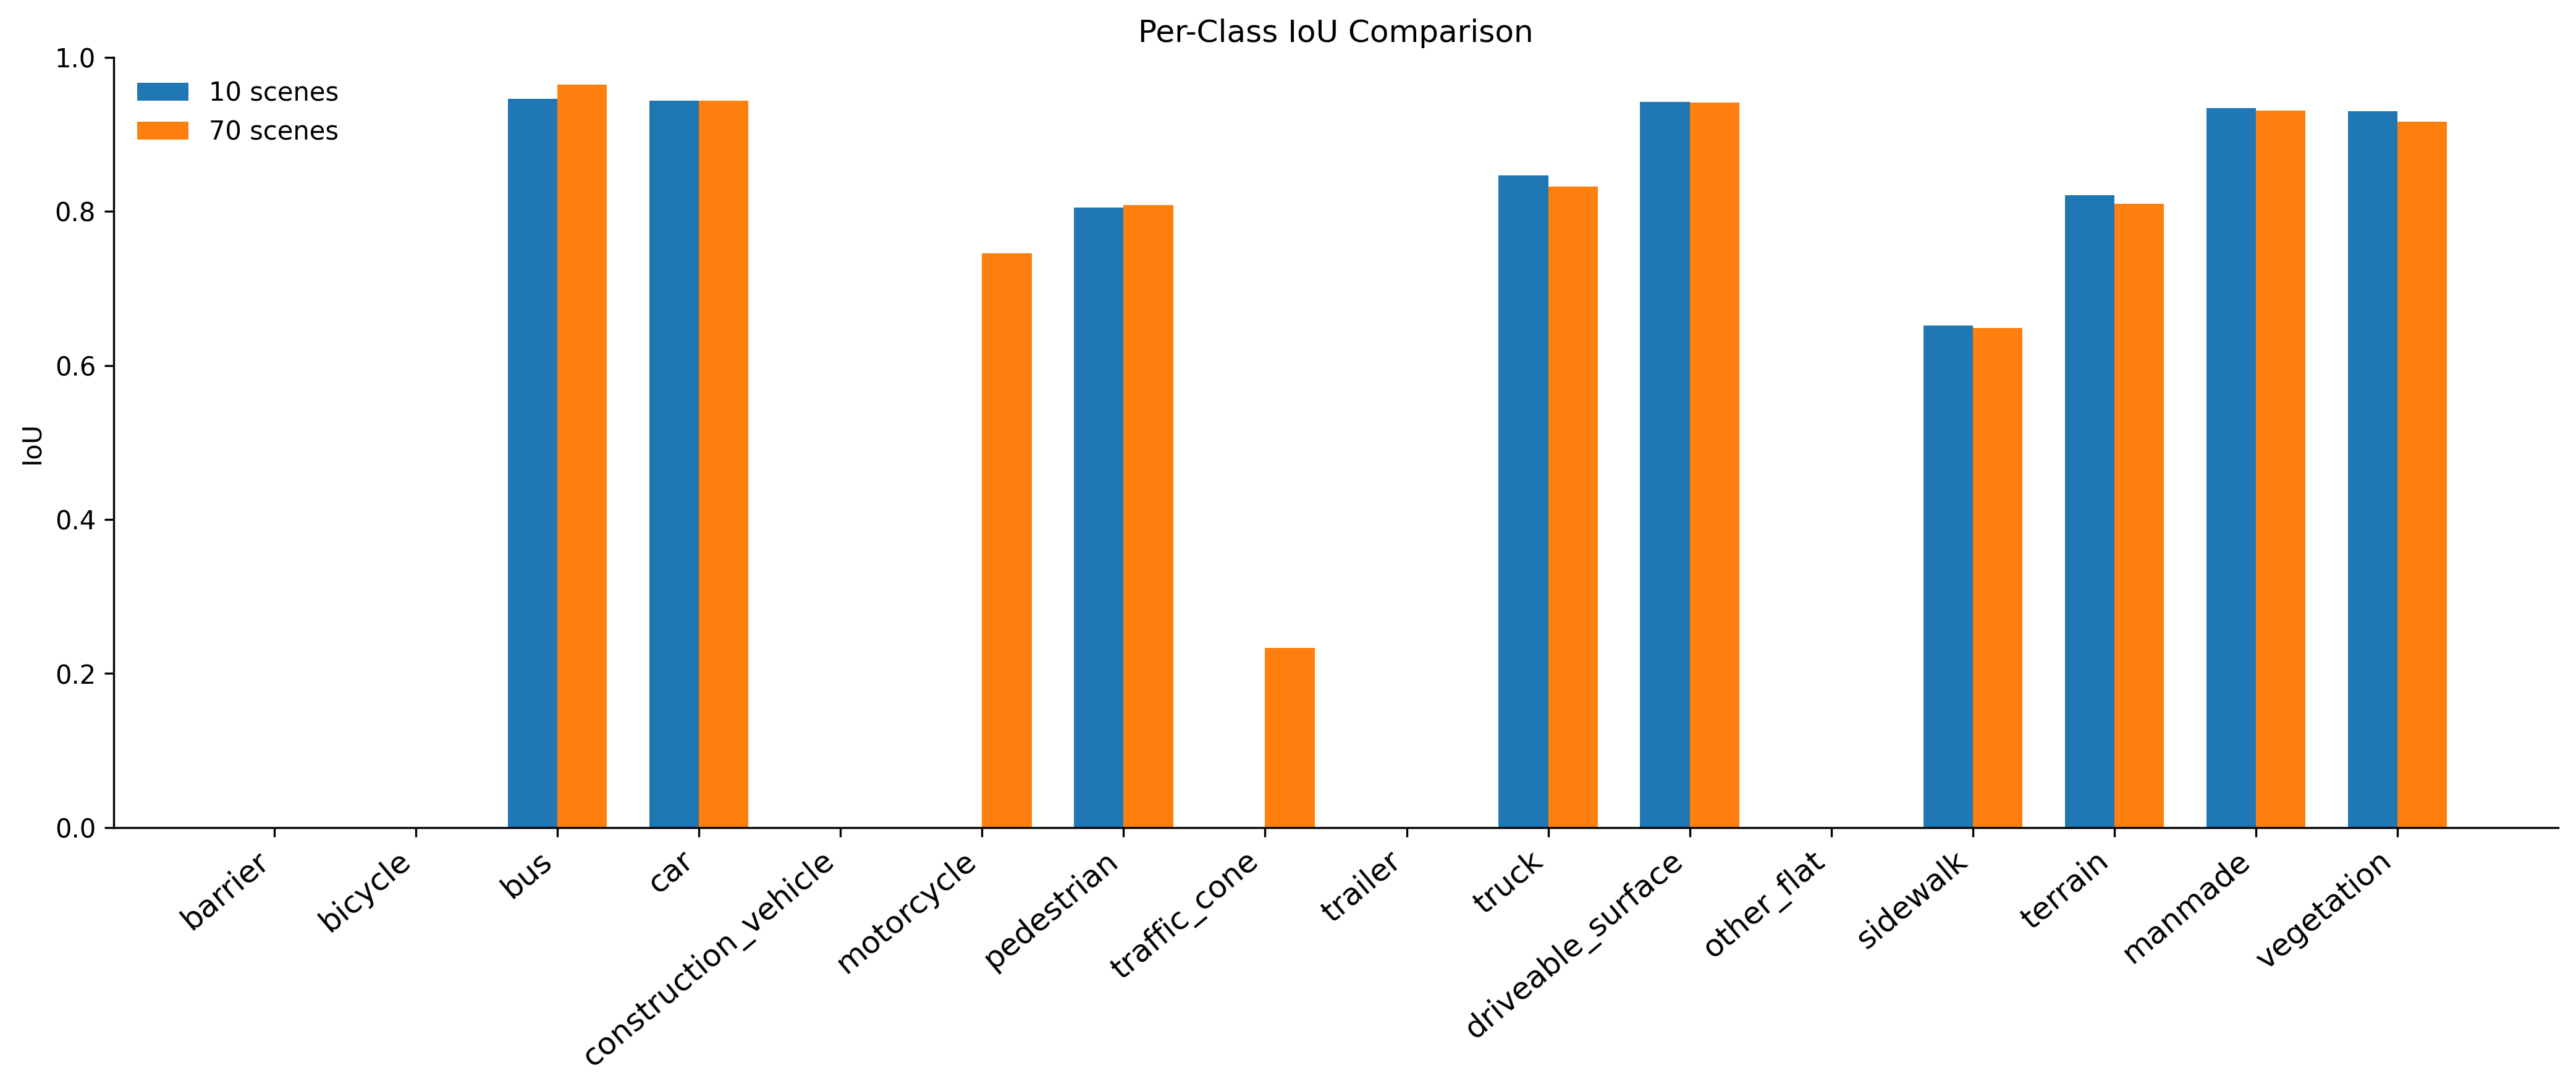
\includegraphics[width=0.9\linewidth]{train_size_figures/per_class_iou.png}
\caption{mIoU for $10$ scenes vs.\ $70$ scenes at $\lambda=0.0$ on the held out nuScenes mini validation split for each semantic category.}
\label{fig:10vs70class}
\end{figure*}

\end{document}
